\section{Communication Filtering}
The GoT positioning system gives the vehicle's coordinates throughout time that have to be sent through radio waves. However, since this system functions with ulrasound waves to register positions in space, these can easily be distorted by interferences and objects on the wave path. It is therefore required to eliminate big jumps that could happen in the GoT coordinates before sending them to the vehicle, see \chapref{Requirements}.

Since the vehicle cannot run faster than \si{3,0\ m \cdot s^{-1}} and that the chosen velocity for the velocity controller is \si{1,4\ m \cdot s^{-1}}, it is possible to define a certain range of positions during a wanted interval. This positions' set define a circle of radius as large as the assumed maximum velocity, set to \si{3,0\ m.s^{-1}}, multiplied with the measurement time interval. An example with a \si{1,0\ s} interval is given on \figref{GoTFilterSimple}.
\begin{figure}[H]
  \centering
  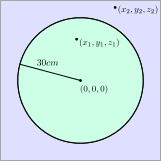
\includegraphics[scale=0.6]{figures/GoTFilterSimple.pdf}
  \caption{Disk of possible positions for a maximum speed of \si{3,0\ m \cdot s^{-1}} during a \si{1\ s} interval}
  \label{GoTFilterSimple}
\end{figure}
If the position at a given time, \si{t_0} is \si{(0,0,0)}, the coordinates at the next measurement time, \si{t_1\ =\ t_0\ +\ 1\ s}, should stay within a \si{3,0\ m} radius.

To ensure the fact that no coordinate jump is sent to the vehicle, its velocity is measured from the two last sets of coordinates (converted from \si{mm} to \si{m}) and the sampling time of the GoT system (\si{100\ m \cdot s^{-1}}, see \secref{GoTDescription}), see \eqref{eq:velocityGoTCalc}.
\begin{flalign}
\eq{v}{\frac{\sqrt{(X_{2} - X_{{1}})^2 + (Y_{2} - Y_{{1}})^2 + (Z_{2} - Z_{{1}})^2}}{\Delta T}}\unit{m \cdot s^{-1}}
\label{eq:velocityGoTCalc}
\end{flalign}
\hspace{6mm} Where:\\
\begin{tabular}{p{1cm}lll}
  &\si{v}                   & is the velocity of the vehicle                      &\unitWh{m \cdot s^{-1} }\\
  &\si{(X_{2},Y_{2},Z_{2})}   & is the the last set of measured coordinates         &\unitWh{m}\\
  &\si{(X_{1},Y_{1},Z_{1})}   & is the the second last set of measured coordinates  &\unitWh{m}\\
  &\si{\Delta T}            & is the sampling time                                &\unitWh{s}\\
\end{tabular}

Whenever a calculated velocity is greater than the limit of \si{3,0\ m \cdot s^{-1}}, the newest set of coordinates is completely discarded. To calculate the newest velocity again, the previous good set and the very last one are taken, and the sampling time is extended by \si{100\ m \cdot s^{-1}} until a correct velocity is measured and this time interval is reset to the default value.

However, this type of inconsistency in the data should be fairly rare at a speed of \si{1,4\ m \cdot s^{-1}} when the GoT is correctly calibrated and the vehicle's environment is clear of interfering obstacles.